%%%%%%%%%%%%%%%%%%%%%%%%%%%%%%%%%%%%%%%%%%%%%%%%%%%%%%%%%%%%%%%%%%%%
%% I, the copyright holder of this work, release this work into the
%% public domain. This applies worldwide. In some countries this may
%% not be legally possible; if so: I grant anyone the right to use
%% this work for any purpose, without any conditions, unless such
%% conditions are required by law.
%%%%%%%%%%%%%%%%%%%%%%%%%%%%%%%%%%%%%%%%%%%%%%%%%%%%%%%%%%%%%%%%%%%%

% This theme was based on fibeamer theme 
% If you found any bugs please contact @karlosos
% This repository is hosted on github https://github.com/karlosos/zut-fibeamer/

\documentclass{beamer}
\usetheme[faculty=wi]{fibeamer}
\usepackage[utf8]{inputenc}
\usepackage[
  main=portuguese,
  english
]{babel}

\title{Sistema de Monitoramento de Qualidade de Imunobiológicos na Cadeia de Distribuição e Armazenamento}
\subtitle{Henrique M. Miranda}
\author{}

\usepackage{ragged2e}  % `\justifying` text
\usepackage{booktabs}  % Tables
\usepackage{tabularx}
\usepackage{tikz}      % Diagrams
\usetikzlibrary{calc, shapes, backgrounds}
\usepackage{amsmath, amssymb}
\usepackage{url}       % `\url`s
\usepackage{listings}  % Code listings
\frenchspacing
\begin{document}
\frame[c]{\maketitle}

\AtBeginSection[]{% Print an outline at the beginning of sections
  \begin{frame}<beamer>
    \frametitle{Seção \thesection}
    \tableofcontents[currentsection]
  \end{frame}
}

\begin{darkframes}
  \section{Dark Frames}
  \begin{frame}{Jabberwocky}
    \framesubtitle{Lewis Carroll}%
    \begin{tikzpicture}[overlay,remember picture]
      \node[anchor=south east,xshift=-30pt,yshift=35pt]
      at (current page.south east) {
        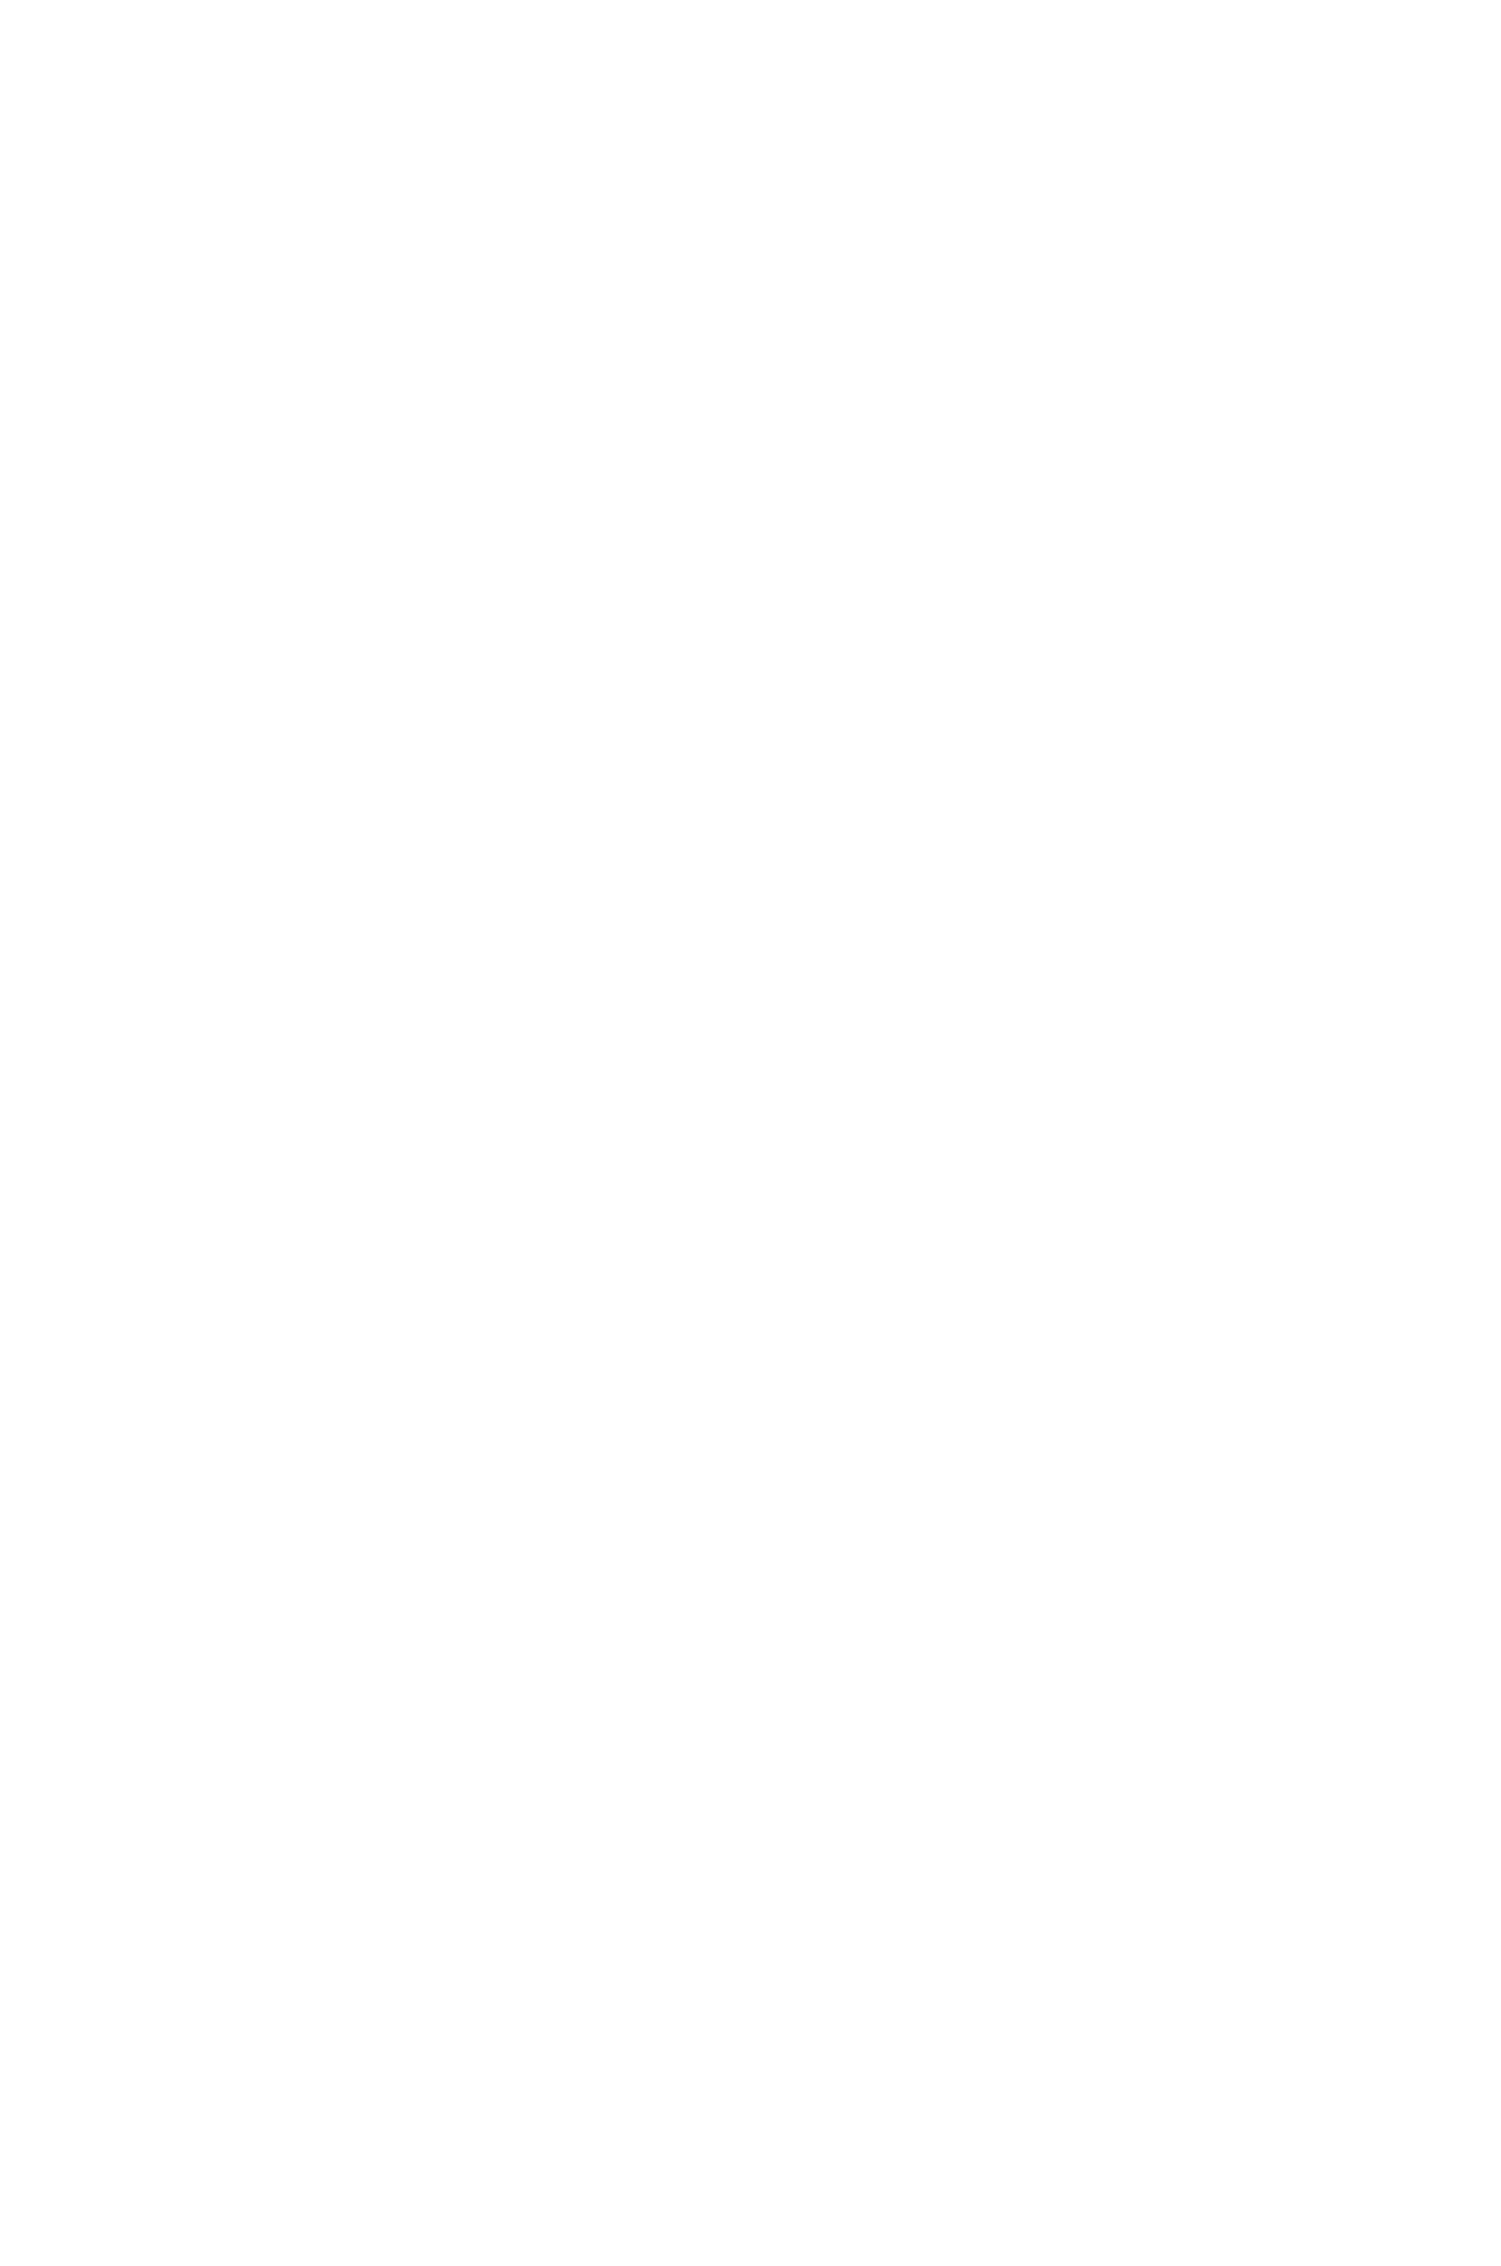
\includegraphics[width=35mm]{resources/jabberwocky-dark}
      };
    \end{tikzpicture}%
    'Twas brillig, and the slithy toves\\
    Did gyre and gimble in the wabe;\\
    All mimsy were the borogoves,\\
    And the mome raths outgrabe.\\\bigskip

    “Beware the Jabberwock, my son!\\
    The jaws that bite, the claws that catch!\\
    Beware the Jubjub bird, and shun\\
    The frumious Bandersnatch!”\\
  \end{frame}
\end{darkframes}
\end{document}
